\documentclass[12pt, titlepage, oneside]{article}

\usepackage[margin=1in]{geometry}
\usepackage{siunitx, booktabs, amsmath, enumitem, pdfpages,mathrsfs,tabularx,caption, graphicx, pgfplots, textcomp,wrapfig, commath, svg, amsfonts, relsize}
\usepackage{parskip}
\usepackage[siunitx]{circuitikz}
\sisetup{detect-weight=true, detect-family=true}
\renewcommand{\vec}[1]{\oldvec{\bm{#1}}}
\renewcommand{\hat}[1]{\oldhat{\bm{#1}}}
\renewcommand{\b}[1]{\textbf{#1}}
\newcommand{\de}[1]{\noindent\fbox{\parbox{\textwidth}{#1}}}



\newcommand{\items}{\begin{itemize}}
\newcommand{\eitems}{\end{itemize}}


\newcommand{\ex}{Ex. }
\newcommand{\exe}{_}

\newcommand{\n}{\cap}
\renewcommand{\u}{\cup}


\begin{document}
	
	\textbf{ELECENG 3TQ3}\\
	\textbf{Elston A.}
	
	\section{Lecture 1}

\subsection{Probability vs. Statistics}

\items
\item Statistics is probability formulate differently
\item Statistics applies to probability to extract information about data and recommend what decisions should be made
\eitems

\b{Probabilistic: } You have a fair coin, you flip it 100 times, what is the probability to getting more than a 70\% heads (We expect a small number).

\b{Statistical: } You have a coin of unknown fairness, you flip it 100 times and get 70\% heads. Your job would be to draw conclusions about that coin. 

The main difference is that you know the conditions when you are deriving probability of a particular outcome. In statistics, you know the outcome and you are trying to obtain conclusions about the underlying relations, models, and hidden patterns in the data.

\subsection{Frequency vs. Bayes}

Consider a simple coin toss and assume you toss it $n$ times. Let $nh$ be the number of heads and $nt = n - nh$ be the number of tails.

The \b{Frequentist} estimates the probability of heads as $Ph = nh/n$. That is the frequency of the "head" event.

The \b{Beyesian} attempts to find prior knowledge such as where was the coin minted and built. This "prior" information is then used for analyzing the data.

\subsection{Counting and Sets}

We need to determine all the possible all the outcomes in order to determine probabilities. To accomplish this we would need to understand sets, unions, intersections, and complements. Also aspects of of combinatorics calculus is needed in order to analyze problems eg. selecting $n$ out of $m$ objects.

\ex Toss a fair coin 4 times. What is the probability to get exactly two tails? 

We can approach this using the counting approach by finding all the possible outcomes.

S = \{ HHHH, HHHT, HHTH, HHTT, HTHH, HTHT, HTTH, HTTT, THHH, THHT, THTH, THTT, TTHH, TTHT, TTTH, TTTT\}

Then we find the set of favorable outcomes

A = \{HHTT, HTHT, HTTH, THHT, THTH, TTHH\}

So the probability of the event to exactly two tails in 4 tosses is the number of favourable outcomes divided by the total outcomes = 6/16.

But this type of approach becomes impossible once the space grows. \ex if we had 100 tosses. 
	
\subsection{Formalizing Sets/Counting}

A \b{set} is a collection of elements: \ex patients with blood pressure over 140, people with brown hair, etc.

We use $x \in S$ to denote \b{element} x belonging to the set $S$: \ex John has brown hair, hence John is an element in the set of people with brown hair.

We say a set $A$ is a \b{subset} of $S$ if all the elements in $A$ belongs to $S$: \ex we can pick 6 people from the people with brown hair set and make a new set. This new set would be a subset of the original set of people with brown hair.

An \b{empty set} is the set with no elements denoted as $\emptyset$

\subsection{Set Operations}

\b{Complement}: The complement of $A$ in $S$ is all the elements in $S$ that are not in $A$. We denote this as $S-A$ or $A^c$. 

\ex Let $B$ be the set of all the people with brown hair and shorter than 6 feet. The complement of this would be all the people who do not have brown hair or are taller than 6 feet. 

\b{Union}: The union of $A$ and $B$ is the set of all the elements that are in $A$ or $B$ (or in both). We denote this as: $A \u B$.

\b{Intersection}: The intersection of $A$ and $B$ is the set of all elements that are in both $A$ and $B$. We denote this as: $A\n B$.

\b{Disjoint}: Two sets are called disjoint if they have no mutual elements

\b{Difference}: The difference of $A$ and $B$ is the set of all elements in A, but are not in B and is denoted as $A \backslash B$.

\ex Consider a set of 10 cities \{Berlin, Munich, Madrid, Barcelona, Beijing, Shanghai,  Portland, Washington DC, Ottawa, Toronto\}

Consider two subsets: 1) M is a set of capitols and 2) N is a set of cities in Europe

M=\{Berlin, Madrid, Beijing, Washington DC, Ottawa\}

N=\{Berlin, Munich, Madrid, Barcelona\}

\items
\item Intersection: \{Berlin, Madrid\}
\item Union: \{Berlin, Munich, Madrid, Barcelona, Beijing, Washington DC, Ottawa\}
\item Complement of M in S : \{Munich, Barcelona, Shanghai, Portland, Toronto\}
\item Difference  = \{Beijing, Washington DC, Ottawa\}
\eitems


\subsection{De Morgans Laws}

\begin{align}
(A \u B)^c = A^c \n B^c
\end{align}
\begin{align}
(A \n B)^c = A^c \u B^c
\end{align}



\subsection{Proof of De Morgans Laws}

\begin{align*}
&x \in (A \n B)^c\\
&\iff x \notin (A \n B) \\
&\iff x \in A^c \u x \in B^c
\end{align*}
\begin{align*}
&x \in (A \u B)^c\\
&\iff x \notin (A \u B)\\
&\iff x \in A^c \n x \in B^c
\end{align*}

\subsection{Venn Diagrams}


 \begin{figure}[h!]
 	\centering
 	
\includegraphics[width=0.5\linewidth]{images/S}
 	\caption{Set $S$ of all possible outcomes}
 	\label{fig:s}
 \end{figure}
 \begin{figure}[h!]
 	\centering
 	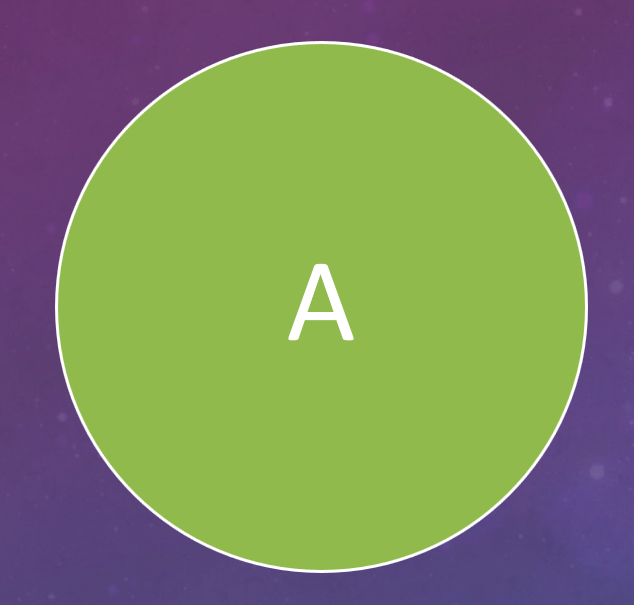
\includegraphics[width=0.2\linewidth]{images/A}
 	\caption[]{The set of all the outcomes in $A$}
 	\label{fig:a}
 \end{figure}
 
 \begin{figure}[h!]
 	\centering
 	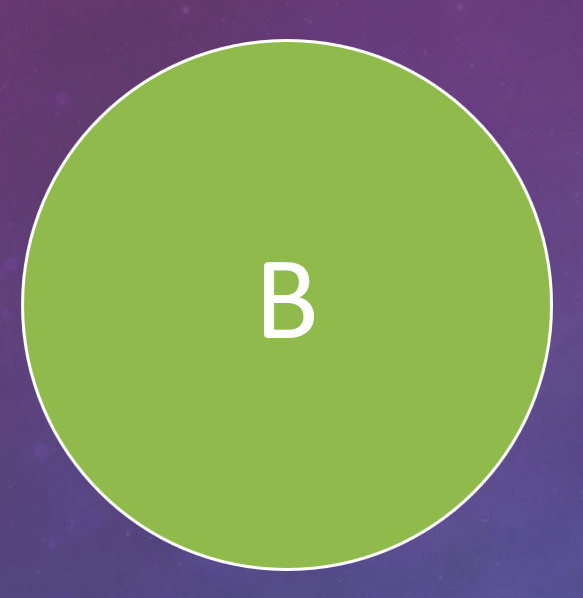
\includegraphics[width=0.2\linewidth]{images/B}
 	\caption[]{The set of all the outcomes in $B$}
 	\label{fig:b}
 \end{figure}
 
 \begin{figure}[h!]
 	\centering
 	
\includegraphics[width=0.3\linewidth]{images/Union}
 	\caption[]{Union of set $A$ and set $B$}
 	\label{fig:union}
 \end{figure}
 
\begin{figure}[h!]
	\centering
	
\includegraphics[width=0.2\linewidth]{images/intersection}
	\caption{Intersection of $A$ and $B$}
	\label{fig:intersection}
\end{figure}

\begin{figure}[h!]
	\centering
	
\includegraphics[width=0.3\linewidth]{images/Ac}
	\caption{Complement of $A$ or $A^c$}
	\label{fig:ac}
\end{figure}
\newpage 
\begin{figure}[h!]
	\centering
	
\includegraphics[width=0.3\linewidth]{images/B-A}
	\caption{$B-A$ or $B \backslash A$}
	\label{fig:b-a}
\end{figure}

\subsection{Set Product and Additional Set Terminology}

$S \times T = \{ (s,t) \in S \text{ and } t \in T\}$

\ex $\{1,2\} \times \{3,4,5\} = \{(1,3),(1,4),(1,5), (2,3), (2,4), (2,5)\}$

Cardinal number is the number of elements in the set. Cardinal number is denoted as $\#s$ or $card\{S\}$ or $|S|$.

Inclusion - Exclusion principle: $|A \u B| = |A| + |B| - |A \n B| $ 

We subtract $|A \n B|$ to ensure we do not double count.

\end{document}